\chapter{Anforderungen}
\section{Benutzer und Personas}
Die Benutzer der Project Helin Plattform teilen sich in drei Gruppen auf, welche in dieser Arbeit berücksichtigt werden. Die Gruppen werden nach der primären Funktion unterschieden.
\begin{itemize}
	\item{\textbf{Kunde:} Der Kunde hat primär Interesse an einem Produkterwerb. Er möchte Projekt Helin als Transportplattform für seinen Auftrag verwenden. Er besitzt weder eine Drohne noch ein passendes Geschäftsmodel, welches eine Drohne nutzen möchte.}
	\item{\textbf{Administrator:} Administratoren verwenden die Project Helin Plattform um eine Flotte von Drohnen zu verwalten. Sie nutzen dazu die Webseite der Plattform und kümmern sich um das Definieren von Flugzonen, Services und Gütern.}
	\item{\textbf{Drone-Operator:} Der Drone-Operator kümmert sich primär um die Drone und verwendet dafür die Onboard-App um die Drohne einem Organisationsinventar hinzuzufügen.}
\end{itemize}
\subsection{Persona Diego: Kunde}
\begin{figure}[h]
\centering
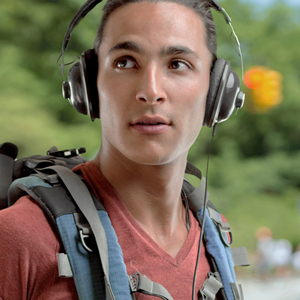
\includegraphics[width=0.35\textwidth]{images/persona-diego.jpg}
\caption{Persona Diego: Freie Lizenz; Quelle 
\protect\url{http://blog.placeit.net/free-avatar-pack/}}
\label{fig:diego}
\end{figure}
Diego ist \textbf{23 Jahre alt} wohnt in einer WG in Uster.
Diego hat eine Informatik-Lehre mit BMS abgeschlossen und ist auf der Suche nach einer neuen beruflichen oder schulischen Herausforderung.
\paragraph{Technisches Verhalten}
Arbeitet täglich acht Stunden mit dem PC. Nutzt gerne neue Technologien. Besitzt ein Android-Smartphone der neusten Generation. Die Android Updates macht er immer sofort. Interessiert sich für neue Technologien und sieht sich regelmässig Kickstarter Projekte an.
\paragraph{Ziele}
Möchte sich weiterbilden und neue Herausforderungen finden. Möchte neue Technologien entdecken und einsetzen.
\paragraph{Szenario}
Diego möchte an einem Openair frisches Bier für sich und seine Frenude bestellen, er hat aus der Zeitung von Projekt Helin erfahren und möchte aufgrund seines technischen Interesses den Dienst in Anspruch nehmen.
\subsection{Persona Carmen: Administratoren}
\begin{figure}[h]
\centering
	
\includegraphics[width=.35\textwidth]{images/persona-stefanie.jpg}
	\caption{Persona Stefanie: Freie Lizenz; Quelle
	 \protect\url{http://blog.placeit.net/free-avatar-pack/}}
	\label{fig:stefanie}
\end{figure}
Carmen ist \textbf{35 Jahre alt} und lebt alleine in Zürich.
Sie unternimmt viel mit Freunden und reist gerne. Sie ist auf dem Land aufgewachsen und wohnt jetzt in Zürich.
Carmen arbeitet bei einer Eventagentur und hat eine Ausbildung als Eventmanagerin abgeschlossen.

\paragraph{Technisches Verhalten}
Sie nutzt den PC täglich bei der Arbeit, vor allem Planungstools und das E-Mail-Programm. Ausserdem ist sie zu Recherchezwecken viel im Internet unterwegs. Sie nutzt Chrome als Browser im Geschäft. Sie besitzt ein Samsung Galaxy S4, dass sie schon seit einigen Jahren verwendet. Zuhause hat sie keinen PC.
\paragraph{Kommunikationsverhalten}
Sie kommuniziert geschäftlich hauptsächlich per E-Mail. Mit Freunden unterhält sie sich oft über WhatsApp.
\paragraph{Ziele}
Sie möchte mit neuen und innovativen Ideen Events für Besucher spannender gestalten.

\subsection{Persona Ricardo: Drone Operator}
\begin{figure}[h]
\centering
	
\includegraphics[width=.35\textwidth]{images/persona-ricardo.jpg}
	\caption{Persona Ricardo: Freie Lizenz; Quelle
	 \protect\url{http://blog.placeit.net/free-avatar-pack/}}
	\label{fig:ricardo}
\end{figure}
Ricardo ist 26 Jahre alt und wohnhaft in Wetzikon. Der ausgebildete Schlosser hat zur Zeit keinen festen Job. Er lebt das Leben von Tag zu Tag und geniest es keine festen Verpflichtungen zu haben.
\paragraph{Technisches Verhalten}
Er nutzt den PC selten, vorallem aber zum Surfen im Internet. Als Mobiltelefon besitzt er ein altes Telefon mit Android. Er möchte sich auch kein neues Gerät kaufen, da er ausser Whatsapp und der Taschenlampe das Gerät sowieso nicht verwendet.
\paragraph{Kommunikationsverhalten}
Er verwendet hautpsächlich Email und sein Mobiltelefon zur Kommunikation. Mit Freunden unterhält sie sich auch oft über WhatsApp.
\paragraph{Ziele}
Ricardo möchte gerne am Openair etwas Geld dazu verdienen und ohne grosse Einarbeitungszeit den Anforderungen der Eventtechnikfirma genügen.
\newpage
\section{Funktionale Anforderungen}

Die funktionalen Anforderungen leiten sich aus der Aufgabenstellung, sowie den mit dem Betreuer diskutierten Ideen ab.

\subsection{Administrator}
\begin{itemize}
\item Als Administrator möchte ich auf der Webseite einen Account erstellen können.
\item Als Administrator möchte ich ein Projekt erfassen können.
\item Als Administrator möchte ich auf eine Drohne dem Projekt hinzufügen können.
\item Als Administrator möchte ich alle Drohnen verwalten können (RUD).
\item Als Administrator möchte ich Güter verwalten können (CRUD).
\item Als Administrator möchte ich Services verwalten können (CRUD). (optional)
\item Als Administrator möchte ich Flug-, Lade- und Abwurfzonen verwalten können.
\item Als Administrator möchte ich Bestellungen verwalten können (CRUD).

%add where - what de fuck is a mission mst, 01.04.2016

\item Als Administrator möchte ich Missionen vor, nach, und während der Ausführung ansehen können.
\item Als Administrator möchte ich Missionen abbrechen können.
\end{itemize}

\subsection{Kunde}
\begin{itemize}
\item Als Kunde möchte ich eine App aus dem Google Play Store herunterladen können.
\item Als Kunde möchte ich die App nutzen ohne mich anmelden zu müssen.
\item Als Kunde möchte ich in der App, aus einer Liste von Gütern und Services, eine Auswahl treffen können.
\item Als Kunde möchte ich eine Bestellung tätigen können.
\item Als Kunde möchte ich die bestellte Ware direkt bezahlen können. (optional)
\item Als Kunde möchte ich auf der Karte des Smartphones die Bewegung der Drohne verfolgen können.
\item Als Kunde möchte ich textuelle Updates über den Status meiner Bestellung erhalten.
\item Als Kunde möchte ich eine Bestellung stornieren können.
\end{itemize}

\subsection{Drone-Operator}
\begin{itemize}
	\item Als Drone-Operator möchte ich eine Android App mit Hilfe der heruntergeladenen APK installieren können.
	%APK in GLOSSAR!
	\item Als Drone-Operator möchte ich das Gerät bzw. die Drohne beim Server registrieren können.
	\item Als Drone-Operator möchte ich das Gerät bzw. die Drohne zu einer Organisation hinzufügen können.
	\item Als Drone-Operator möchte ich das OTG-Fähige Smartphone an einen MAV-Link kompatiblen Flight-Controller über USB anschliessen können.
	\item Als Drone-Operator möchte ich eine Verbindung zwischen App und Server über das Internet herstellen könnnen.
	\item Als Drone-Operator möchte ich eine Verbindung zwischen App und Flight-Controller herstellen können.
	\item Als Drone-Operator möchte ich den aktuellen Zustand der Verbindungen zur Drohne und zum Server sehen.
	\item Als Drone-Operator möchte ich den aktuellen Status des Flight-Controllers, beispielsweise GPS und Batteriespannung sehen.
	\item Als Drone-Operator möchte ich sehen wenn der Drohne eine neue Mission zugeteilt wurde.
	\item Als Drone-Operator möchte ich eine Liste von Gütern anzeigen lassen, die für die aktuelle Mission geladen werden müssen.
	\item Als Drone-Operator möchte ich eine Mission annehmen oder ablehnen können.
	\item Als Drone-Operator möchte ich die Beladung einer Drohne bestätigen können.
	\item Als Drone-Operator erhalte ich ein visuelles und akustisches Countdown-Signal bevor die Drohne startet.
	\item Als Drone-Operator möchte ich den Start der Drohne während des Countdowns verhindern können.
\end{itemize}
\newpage
\section{Nichtfunktionale Anforderungen}
\subsection{Verbindungsabbruch}
\begin{tabular}{|p{.25\textwidth}|p{.75\textwidth}|} \hline
	Synopsis & Verbindungsabbruch der Onboard App zum Server soll keine negativen Auswirkungen auf die Mission haben.  \\ \hline
		
	Messbarkeit & Nach dem Start der Mission muss die Drohne auch ohne Verbindung zum Server die Mission abschliessen können. \\ \hline
\end{tabular}

\subsection{Sicherheit im Mittelpunkt}
\begin{tabular}{|p{.25\textwidth}|p{.75\textwidth}|} \hline
	Synopsis & Eine Drohne führt vor dem Freigeben der Motoren (Arming) einen Check durch, der prüft ob alle nötigen Voraussetzungen für einen Start erfüllt sind. Ausserdem müssen vor einem Start ebenfalls Voraussetzungen der Mission erfüllt sein, beispielsweise muss der Drone-Operator den Start freigeben. Sollte eine dieser Vorraussetzungen nicht erfüllt sein, darf die Drohne nicht starten.  \\ \hline
	
	Messbarkeit & Drohne darf nicht starten, falls der Pre-Flight-Check des Autopiloten nicht erfolgreich war oder Voraussetzungen für die aktuelle Mission nicht erfüllt sind. \\ \hline
\end{tabular}
\subsection{Verbindungswiederherstellung}
\begin{tabular}{|p{.25\textwidth}|p{.75\textwidth}|} \hline
	Synopsis & Nach einem Verbindungsabbruch zwischen dem Server und der Onboard App soll die Verbindung wiederhergestellt werden sobald wieder Internet verfügbar ist. \\ \hline
	
	Messbarkeit & Die Verbindung zwischen Server und App wird nach dem deaktivieren und wieder aktivieren der Internetverbindung innert 30 Sekunden wiederhergestellt.\\ \hline
\end{tabular}
\subsection{Nutzlast der Drohne}
\begin{tabular}{|p{.25\textwidth}|p{.75\textwidth}|} \hline
	Synopsis & Eine 1/2 Liter PET Flasche soll innerhalb von einem 500m Radius geliefert werden können. \\ \hline
	Messbarkeit & Im App kann ein Produkt mit einem Gewicht von 500g bestellt, und geliefert werden. \\ \hline
\end{tabular}
\subsection{Security}
\begin{tabular}{|p{.25\textwidth}|p{.75\textwidth}|} \hline
	Synopsis & Es darf nicht möglich sein, dass jemand die Steuerung einer beim Server registrierten Drohne übernehmen kann.\\ \hline
	Messbarkeit & Der Übertragungskanal vom Server zur Drohne muss verschlüsselt sein und es dürfen sich keine weiteren Producer anmelden können.\\ \hline
\end{tabular}
\section{Domain-Model}
Aus den funktionalen Anforderungen ergibt sich das folgende Domainmodel.
\begin{landscape}
\begin{figure}[h]
	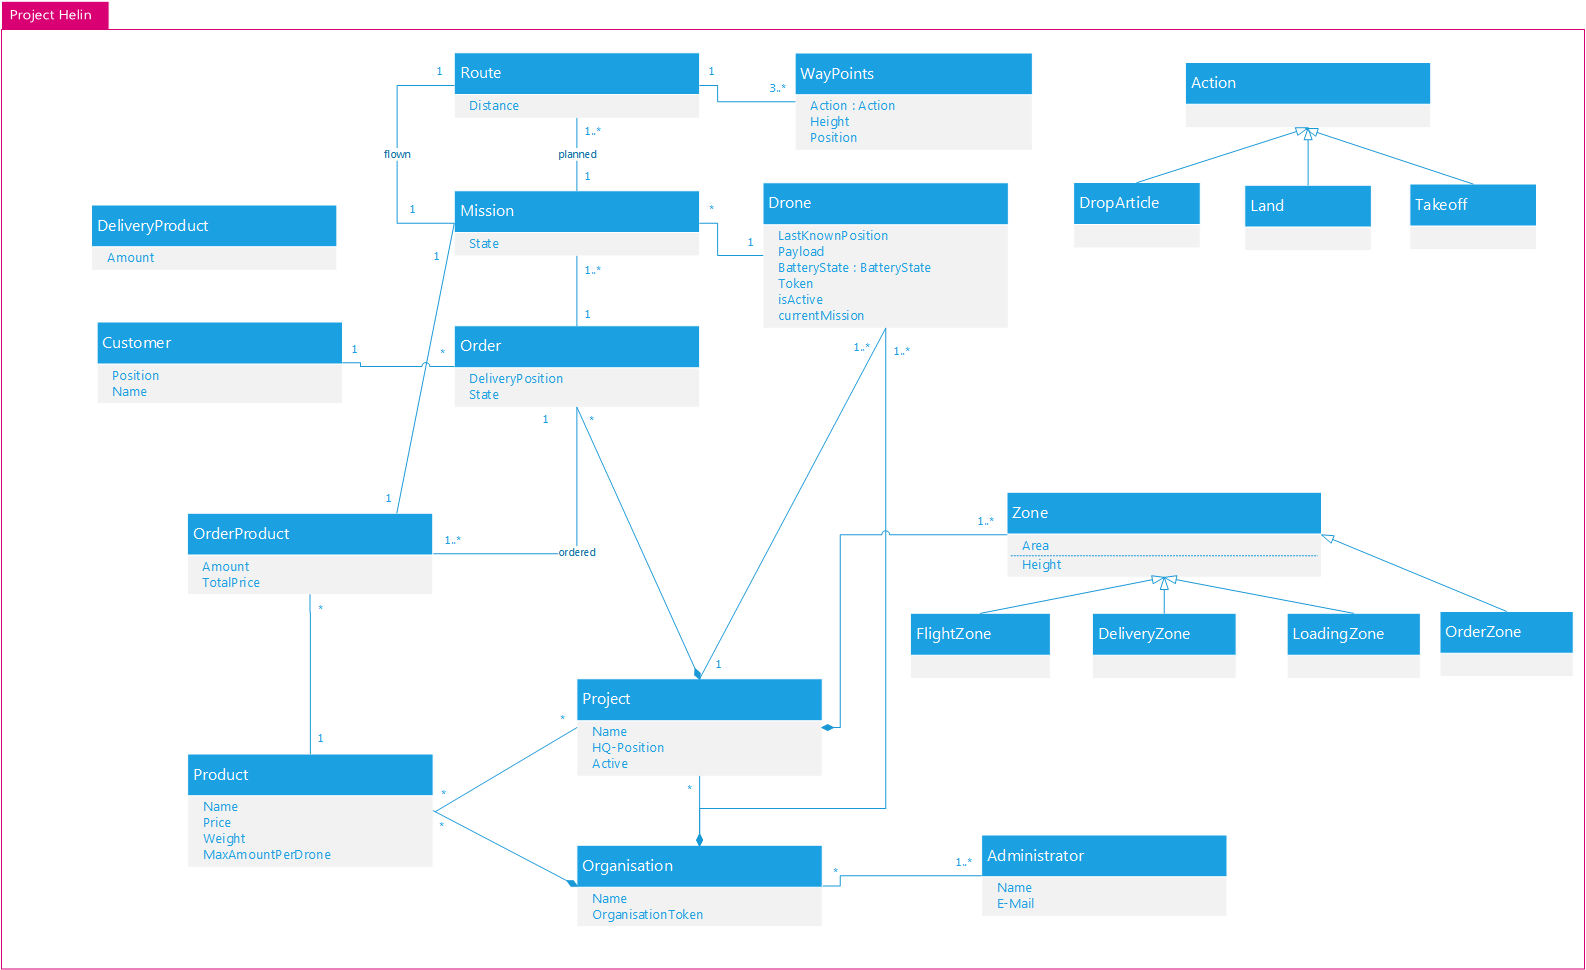
\includegraphics[width=0.75\paperheight]{images/domainmodell.png}
	\caption{Domain-Model}
	\label{fig:domain-model}
\end{figure}
\end{landscape}

